%\newpage
In this chapter, we first introduce some widely used convolutional operations,  some examples of convolution filters and their performance, and then some popular convolutional neural network (CNN) models.
\section{Convolutional operations}

\subsection{Images as matrix}\label{sec:functions}
An image can be viewed as a piecewise constant function on a grid.  Images with different
resolutions can then be viewed as functions on grids of different
sizes.  The use of such multiple-grids is a main technique used in the
standard multigrid method for solving discretized partial differential
equations, and it can also be interpreted as a main ingredient used in
convolutional neural networks (CNN) for image calssification.

An image can be viewed as a function on a grid \cite{krizhevsky2012imagenet} on 
a rectangular  domain $\Omega\in \mathcal R^2$.  Without loss of generality,
 we assume that the grid, $\mathcal T$, is of size
$$
m=2^{s}, \quad n=2^{t} 
$$
for some integers $s, t\ge 1$.
Starting from $\mathcal T_1=\mathcal T$,  we consider a sequence of
coarse grids with $J=\min (s,t)$ (as depicted in Fig.~\ref{mugrid-bi} with $J=4$):
\begin{equation}
\label{grids}
\mathcal T_1, \mathcal T_2, \ldots, \mathcal T_J
\end{equation}
such that ${\cal T}_\ell$ consist of $m_\ell\times n_\ell$ grid
points, with 
\begin{equation}
\label{mn-ell}
 m_\ell=2^{s-\ell+1},~~ n_\ell=2^{t-\ell+1}.   
\end{equation}

\begin{figure} \label{mugrid-bi}
\begin{center}
\setlength{\unitlength}{0.445mm}
\begin{picture}(45,45)(50,0)
\linethickness{0.1mm}
\multiput(-20,0)(2.5,0){17}{\line(0,1){40}}
\multiput(-20,0)(0,2.5){17}{\line(1,0){40}}
\multiput(28,0)(5,0){9}{\line(0,1){40}}
\multiput(28,0)(0,5){9}{\line(1,0){40}}
\multiput(77,0)(10,0){5}{\line(0,1){40}}
\multiput(77,0)(0,10){5}{\line(1,0){40}}
\multiput(126,0)(20,0){3}{\line(0,1){40}}
\multiput(126,0)(0,20){3}{\line(1,0){40}}
\end{picture}
\setlength{\unitlength}{0.5mm}
\end{center}
$$ 
\hskip0.05 in \mathcal T_1\hskip 0.7in \mathcal T_2\hskip 0.7in  \mathcal T_3\hskip 0.7in \mathcal T_4
$$
\caption{multilevel grids for piecewise constant functions (images)}
\end{figure}
Here, please note that each element in this grid can be viewed as 
a pixel or an image or an element in a matrix.


\subsection{Convolution operation with one channel}
For simplicity of exposition, we denote 
\begin{equation}\label{eq:size_f}
m = m_1 = 2^{s},  \quad n = n_1 = 2^t.
\end{equation}
Recall the definition of convolution in Definition \ref{def:convolution}.  In image processing, a kernel, convolution matrix, or mask is a small matrix, denoted by $K$ below. It is used for blurring, sharpening, embossing, edge detection, and more. This is accomplished by doing a convolution between a kernel and an image, denoted by $g$ below. Convolution is the process of adding each element of the image to its local neighbors, weighted by the kernel.
\begin{definition}
A convolution defined on $\mathbb{R}^{m\times n}$ is a linear mapping 
$K\ast: \mathbb{R}^{m\times n}\mapsto \mathbb{R}^{m\times n}$ defined with padding,  
for any $g \in \mathbb{R}^{m\times n}$ by:
%We first consider $\theta$ a convolution operator (with stride $1$) 
%and padding:
\begin{equation}\label{con01}
[K \ast g]_{i,j} = \sum_{p,q=-k}^k K_{p, q} g_{i + p, j + q}, \quad i=1:m, j = 1:n.
\end{equation}
\end{definition}
The convolution maps the original  image $g$ to a modified one $K\ast g$ with the same size, and each element $[K \ast g]_{i,j}$ in the resulting image $K\ast g$ is a weighted average of elements in the original image $g$ with weights $K_{p,q}$.
The weights in \eqref{con01} constitute  a kernel matrix
\begin{equation}
K \in \mathbb{R}^{(2k+1) \times (2k+1)},
\end{equation}
where $k$ is often taken as a small integer. 
Here we note that the indices for the entries in $K$ are given in a special way. 
For example, if $k=1, K\in \mathbb R^{3\times 3}$, and 
$$
K=\begin{pmatrix}
	K_{-1,-1} &K_{-1,0} &K_{-1,1} \\
	K_{0,-1} &K_{0,0} &K_{0,1} \\
	K_{1,-1} &K_{1,0} &K_{1,1} \\
	\end{pmatrix},
$$
for we may have the following 2D Laplacian kernel
\begin{equation}\label{key}
K=\begin{pmatrix}
0 &-1 &0\\
-1 &4&-1 \\
0 &-1 &0 \\
\end{pmatrix}.
\end{equation}  
Here padding means how $ g_{i+ p, j + q}$ is defined
when $(i+ p, j + q)$ is out of $1:m$ or $1:n$. 
The following three choices are often used
\begin{equation}\label{eq:padding}
g_{i + p, j + q} = \begin{cases}
0,  \quad &\text{zero padding}, \\
f_{(i + p)\pmod{m}, (s + q)\pmod{n}},  \quad &\text{periodic padding}, \\
f_{|i-1 +p|, |j -1  +q|},  \quad &\text{reflected padding}, \\
\end{cases}
\end{equation}
if 
\begin{equation}
i + p \notin \{1, 2, \dots, m\} ~\text{or} ~  j+ q \notin \{1, 2, \dots, n\}.
\end{equation}
Here $ d \pmod{m} \in \{1, \cdots, m\} $  means the remainder when $d$ is divided by $m$.

Here is a diagram for convolution with one channel (and also stride one).
\begin{figure}[H]
	\begin{center}
		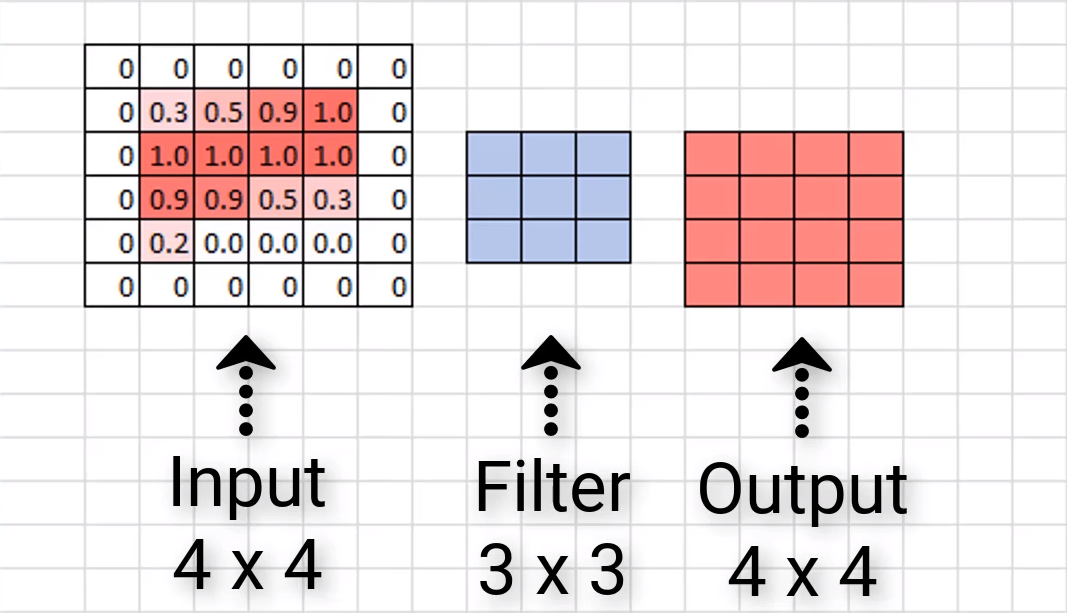
\includegraphics[width=0.5\textwidth]{figures/Conv0padding}
	\end{center}
\end{figure}  
In \cite{bramble1977higher}, the authors show that by ``averaging" the values of 
the finite element solution $u_h$ of elliptic problem using convolution  
 in the neighborhood of a point $x$ they may construct an approximation to the true solution $u(x)$ 
 which is often a better approximation than $u_h(x)$ itself. The ``averaging" operator showed in \cite{bramble1977higher} 
 is just the convolution operator defined here and does not depend on the specific elliptic operator involved.


\subsection{Convolution with stride (one channel)}
Recall the definition  of convolution with stride $2$ in Definition \ref{def:convolution2}, namely,
for $g \in \mathbb{R}^{m\times n}$, convolution with stride $2$ is defined as 
\begin{equation}\label{stride_2}
[K \ast_2 g]_{i,j} = \sum_{p,q=-k}^k K_{p,q} g_{2i + p-1, 2j + q-1},  
\quad i = 1: \lfloor \frac{m+1}{2}\rfloor , j = 1: \lfloor \frac{n+1}{2} \rfloor.
\end{equation} 
Note that the convolution with stride $2$ maps the original image with size $2m\times 2n$ to a new one with smaller size $m\times n$, namely lower resolution.
\begin{lemma}
The convolution with stride $2$ can be written as:
\begin{equation}\label{eq:convstride_2_1}
K \ast_2 g = \mathcal S( K\ast g),
\end{equation}
where $\mathcal S$ is a stride operator defined by:
\begin{equation}\label{eq:strideopdim}
\mathcal S: \mathbb{R}^{m \times n} \mapsto \mathbb{R}^{\frac{m+1}{2} \times \frac{n+1}{2}},
\end{equation}
with
\begin{equation}\label{eq:strideop}
[\mathcal S(g)]_{i,j} = g_{2i-1, 2j-1}, \quad i = 1: \lfloor \frac{m+1}{2}\rfloor , j = 1: \lfloor \frac{n+1}{2} \rfloor.
\end{equation}
\end{lemma}


\begin{example}
The so-called average pooling with kernel size $3 \times 3$ and stride 2 means
\begin{equation}
K \ast_2\quad \mbox{with}\quad
K = \frac{1}{9} 
\begin{pmatrix}
1 & 1 & 1 \\
1 & 1 & 1 \\
1 & 1 & 1
\end{pmatrix}.
\end{equation}
\end{example}







We note that, in general, for any given integer $s\ge1$, a convolution with stride
$s$ for $g \in \mathbb{R}^{m\times n}$  can be  defined as:
	\begin{equation}\label{stride}
	[K \ast_s g]_{i,j} = \sum_{p,q=-k}^k K_{p,q} g_{s(i-1) + p+1, s(j-1) + q+1},  
	\quad i = 1: \lfloor  \frac{m+1}{s}\rfloor, j = 1: \lfloor  \frac{n+1}{s}\rfloor.
	\end{equation}
	Here $ \lfloor  \frac{m}{s}\rfloor$ denotes the biggest integer that less than $\frac{m}{s}$. Similarly, the convolution with stride $s$ maps the original image with size $sm\times sn$ to a new one with smaller size $m\times n$.
	The following is a diagram for stride $2$.
\begin{figure}[H]
\begin{center}
	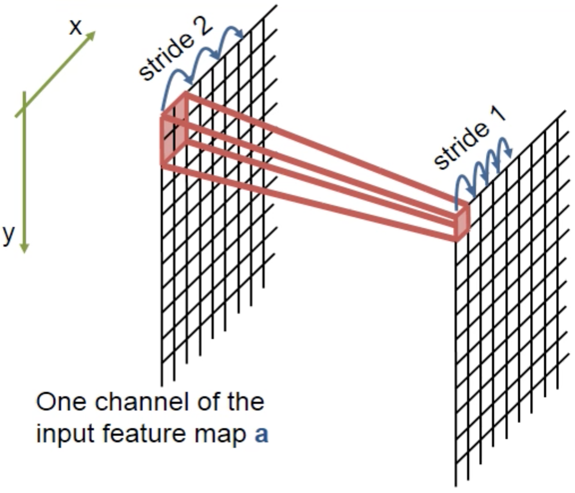
\includegraphics[width=0.35\textwidth]{figures/PoolingLayer1}
\end{center}
\end{figure}

\subsection{Convolutional operations with multi-channel}
In many applications, we need to deal with images with multiple channels. A typical example is the RGB image, where each RGB channel emphasizes different aspects of the original images. Then the inputs become a three-dimensional tensor with size $3\times m\times n$. We refer to this axis, with a size of 3, as the channel dimension. 

When the input data contain multiple channels, we need to construct a convolution kernel with the same number of input channels as the input data, so that it can perform cross-correlation with the input data. 
One important class of linear mapping is the so-called convolution:
$$
\theta: \mathbb{R}^{c\times m\times n} \mapsto \mathbb{R}^{h\times m\times n},
$$
where $m\times n$ is called the spatial dimension or resolution, $c$ and $h$ are corresponding
to input and output channels. Let $f\in \mathbb{R}^{c\times m\times n}$ and the $t$-th channel $[f]_t \in \mathbb{R}^{m\times n}$.
The operation is defined by 
\begin{equation}\label{conv-1}
[\theta(f)]_{s} = \sum_{t=1}^{c}\mathbf{K}_{s,t} \ast [f]_t + b_s
\bm{1}  \in \mathbb{R}^{m\times n}, \quad s = 1:h,
\end{equation}
where $\bm{1}  \in \mathbb{R}^{m\times n} $ is a 
$m\times n$ matrix with all elements being $1$,
and $\mathbf{K}_{s,t}$ is a convolution operator which maps $ [f]_t\in \mathbb{R}^{m\times n}$ to $[\theta(f)]_{s} \in \mathbb{R}^{m\times n}$.
\begin{equation}\label{con1}
[\mathbf{K}_{s,t} \ast [f]_t]_{i,j} = \sum_{p,q=-k}^k K_{s,t; p,q} f_{t; i + p, j + q}, \quad i=1:m, j = 1:n.
\end{equation}
The coefficients kernel $\mathbf{K}_{s,t}$ in \eqref{con1} constitute  a kernel matrix
\begin{equation}
\mathbf{K}_{s,t} \in \mathbb{R}^{(2k+1) \times (2k+1)},
\end{equation}
where $k$ is often taken as small integers. 

Here a more compact notation for multi-channel convolution can be written as
\begin{equation}
\theta(f) = \mathbf{K} \ast f + \mathbf b
\end{equation}
where
\begin{equation}\label{key}
f = \begin{pmatrix}
[f]_1 \\
[f]_2 \\
\vdots \\
[f]_c
\end{pmatrix},
\quad 
\mathbf{K} = \begin{pmatrix}
K_{1,1} & K_{1,2} & \cdots & K_{1,c} \\
K_{2,1} & K_{2,2} & \cdots & K_{2,c} \\
\vdots & \vdots & \ddots& \vdots \\
K_{h,1} & K_{h,2} & \cdots & K_{h,c} 
\end{pmatrix}, 
\quad 
\mathbf b = \begin{pmatrix}
b_1 \bm 1\\
b_2 \bm 1\\
\vdots \\
b_h \bm 1\\
\end{pmatrix}=b\otimes \bm 1.
\end{equation}

Furthermore, we have the following natural extension of convolution with
stride for multi-channel by 
\begin{equation}\label{conv-1}
[\theta(f)]_{s} = \sum_{t=1}^{c}\mathbf{K}_{s,t} \ast_2 [f]_t + b_s
\bm{1}  \in \mathbb{R}^{\tilde m \times \tilde n}, \quad s = 1:h,
\end{equation}
where
\begin{equation}\label{key}
\tilde m = \lfloor \frac{m+1}{2}\rfloor , \quad \tilde n = \lfloor \frac{n+1}{2} \rfloor, 
\end{equation}






\subsection{Pooling operation in CNNs}
When processing images, we want to  gradually reduce the spatial resolution of our hidden representations, aggregating information so that the higher up we go in the network, the larger the receptive field (in the input) to which each hidden node is sensitive.

Finally, we introduce another type of important operation in CNNs -- pooling.
The key purpose for pooling operator is to reduce the spatial resolution of images (features) in a typical CNN models.
Basically, pooling is an operator
\begin{equation}\label{key}
T: \mathbb{R}^{c_1\times m_1\times n_1} \mapsto \mathbb{R}^{c_2 \times m_2\times n_2}.
\end{equation}
where 
\begin{equation}\label{key}
m_2 = \lfloor \frac{m+1}{s}\rfloor , \quad n_2 = \lfloor \frac{n+1}{s} \rfloor, 
\end{equation}
for any choice of $c_2 \ge 1$. Here $s$ is also called the stride in pooling operations. There are generally two types of pooling:

	\paragraph{Convolution with stride $s$ as pooling} In this case, it often happens that
	\begin{equation}\label{key}
	T = R \ast_s, \quad  (s = 2 \text{ for the main case }).
	\end{equation}
	Here $R$ can be learned or fixed such as average pooling as we discussed before.
	
	\paragraph{Nonlinear pooling} The most commonly used nonlinear pooling is called max-pooling, 
	a max pooling with kernel size $(2k+1)\times (2k+1)$ and stride $s$ is is defined as
	\begin{equation}\label{key}
	[R_{\rm max}(f)]_{t; i,j} = \max \{ f_{t;s(i-1) + p+1, s(j-1) + q+1} ~|~ -k \le p,q \le k\},
	\end{equation}
	here $t$ means channel and $c_2 = c_1$ in this case.

Here is an example for max-pooling with kernel size $3\times3$ and stride $3$.
\begin{figure}[H]
\begin{center}
	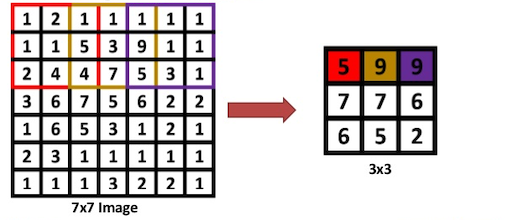
\includegraphics[width=0.5\textwidth]{6DL/figures/3by3MaxPooling}
\end{center}
\end{figure}

\endinput

\subsection{Deconvolution with one channel}
For any linear mapping $\mathcal C: \mathbb{R}^{m\times n} \mapsto \mathbb{R}^{m'\times n'}$, 
its transpose is the unique linear mapping $\mathcal C^\top: \mathbb{R}^{m'\times n'} \mapsto \mathbb{R}^{m\times n}$
satisfying 
$$
(\mathcal C^\top u, v)_{l^2}=(u, \mathcal C v)_{l^2}~~~\forall~u\in \mathbb{R}^{m'\times n'} , v\in \mathbb{R}^{m\times n}
$$
Associated with any kernel $K$, a deconvolution is defined as the transpose of convolution 
with stride $2$ with respect to the $l^2$-inner product as:
\begin{equation}\label{eq:def_deconv}
(u, K \ast_2^\top v)_{l^2}=(K \ast_2 u, v)_{l^2},
\end{equation}
with
\begin{equation}
u \in \mathbb{R}^{m \times n} \quad \text{and} \quad v \in \mathbb{R}^{\frac{m+1}{2} \times \frac{m+1}{2}}.
\end{equation}

\begin{lemma}\label{lemm:tilde-K}
	For any $K \in \mathbb{R}^{(2k+1) \times (2k+1)}$,
	\begin{equation}\label{eq:}
	K\ast_2^\top = {\tilde K}\ast \mathcal S^\top,
	\end{equation}
	where $\tilde K$ is defined as
	\begin{equation}\label{eq:def_tildeK}
	\tilde K_{p,q} = K_{-p, -q}, \quad p,q = -k:k.
	\end{equation}
	Intuitively, if we take $K_{0,0}$ as the center for the convolutional kernel $K$, 
	then $\tilde K$ is the central symmetry of $K$. 
	In 2D case, it can also be understood as the rotation of $\pi$ with respect to
	the center $K_{0,0}$.
\end{lemma}

Recalling the definition of deconvolution in \eqref{eq:def_deconv}, we have
\begin{equation}\label{eq:op_deconv}
\begin{aligned}
(u,  K \ast_2^\top v)_{l^2} &= (K \ast_2 u, v)_{l^2} = (\mathcal S \mathcal C_K u, v)_{l^2} \\
&= (u,  \mathcal C^\top_K \mathcal S^\top v)_{l^2},
\end{aligned}
\end{equation}
with definition
\begin{equation}\label{eq:de_stride_dim}
\mathcal S^\top:   \mathbb{R}^{\frac{m+1}{2} \times\frac{n+1}{2}} \mapsto \mathbb{R}^{m\times n},
\end{equation}
and 
\begin{equation}\label{eq:de_stride}
[\mathcal S^\top (f)]_{i,j} = 
\begin{cases}
0 \quad &\text{if i or j is even}, \\
f_{i/2, j/2}, \quad &\text{else}.
\end{cases}
\end{equation}

Thus to say, we have the simple version of the deconvolution for $K \ast $ as
\begin{equation}\label{eq:simple_deconv}
K \ast_2^\top v = \mathcal C_K^\top \circ \mathcal S^\top (v) = \mathcal C_{\tilde K} \circ \mathcal S^\top (v) = \tilde K \ast \mathcal S^\top (v),
\end{equation}
thus to say
\begin{equation}\label{eq:final}
K \ast_2^\top  = \tilde K \ast \mathcal S^\top.
\end{equation}

In short, we have the next decomposition
\begin{itemize}
	\item convolution with stride = stride $ \circ$ convolution,
	\item deconvolution with stride  = transposed convolution $\circ$ transposed stride = convolution with the central symmetry of original kernel $\circ$ transposed stride.
\end{itemize}

\begin{theorem}\label{thm:deconv_op}
	
	Let us consider 
	\begin{equation}
	K=(K_{p,q}),~~p,q = -1, 0, 1.
	\end{equation}
	Then we have 
	$$
	K \ast_2^\top v = \tilde K \ast \mathcal S^\top (v).
	$$
	As in \eqref{eq:de_stride} and the Lemma \ref{lemm:tilde-K}, we have the 
	final version is 
	\begin{equation}
	\label{eq:7}
	[K \ast_2^\top v ]_{2i,2j}=  K_{0,0}v_{i,j},
	\end{equation}
	with 
	\begin{equation}
	\label{eq:9}
	[K \ast_2^\top v ]_{2i-1, 2j} = K_{0,1}v_{i-1,j} + K_{0,-1}v_{i,j}, \quad 
	[K \ast_2^\top v ]_{2i, 2j-1} = K_{1,0}v_{i,j} + K_{-1,0}v_{i,j-1},
	\end{equation}
	and
	\begin{equation}
	%\begin{tiny}
	%{\scriptsize 
	[K \ast_2^\top v ]_{2i-1, 2j-1}  =  
	K_{1,1}v_{i,j} + K_{-1,1}v_{i-1,j} + K_{1,-1}v_{i,j-1} + K_{-1,-1}v_{i-1,j-1}.
	%\end{tiny}
	%}
	\end{equation}
\end{theorem}
\begin{remark}
	Deconvolution can obviously be also defined for general stride $s$, but we believe it is sufficient to use $s=2$
	in most applications. 
\end{remark}

